\section{Background and Motivation}
\label{sec:background}
\subsection{LFM development}\label{sec:bg_lfm}

 \begin{figure}[!t]
  \centering
  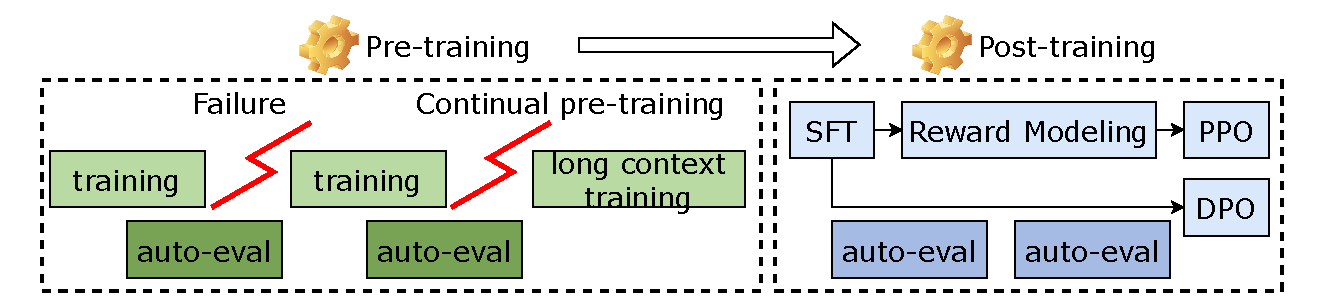
\includegraphics[width=0.95\linewidth]{figures/lfm_pipeline.pdf}
  \caption{
  An overview of the training pipeline of LFM.
  %Separated file systems are used for training data and checkpoint storage. 
  % \yhpeng{make this drawing a bit flatter}
  %Similar pipeline used for other LFMs~\cite{diffusion, dit}.
  }
  \label{fig:lfm_pipeline}
  \vspace{-3mm}
\end{figure}


%\textbf{Clarify the components of LLM checkpoint, its applications in LLM training, and its importance.}
% Checkpoint components and pipeline.
%\noindent \textbf{LFM development.} 
% \yhpeng{Please break down the two stages to include more training phases, e.g., continued training (especially long context training), supervised fine-tuning, reward modeling and reinforcement learning (cite openai-o1). Also visualize these phases in Fig.1} 
% \cwu{make sure all modules in Fig. 1 are explained below}

\noindent \textbf{Production pipeline}.
As depicted in Fig.~\ref{fig:lfm_pipeline}, the development of LFM comprises pre-training and post-training stages.
During the initial pre-training phase, The LFM is iteratively trained on extensive data 
% \cwu{pretraining may not only use unlabeled data}
collected from multiple sources to absorb knowledge about the world. 
Subsequently, continual pre-training is employed to enhance the foundation model's capabilities. 
For instance, the pre-training of large language models (LLMs) typically involves long-context continual training to gradually increase the supported context length of LLMs. 
% while still maintaining their short-context ability.
%are converted into discrete tokens. By iteratively performing the next-token prediction task, LFMs absorb vasts amount of knowledge from the input data.
%Besides, accompanying tasks like 
Post-training is employed to align the pre-trained model with human feedback or enhance the model's reasoning capabilities~\cite{openai-o1, deepseek-r1}.
% generate content that adheres to given instructions~\cite{ppo-framework}.
Various task-specific labeled datasets (\eg, multilingual, code, math, reasoning, etc.) are involved in fine-tuning the LFMs, followed by reinforcement learning, typically including the reward modeling and then performing Proximal Policy Optimization~\cite{ppo} (PPO), or directly conducting Direct Preference Optimization~\cite{dpo} (DPO). 
Due to the reduced size of these datasets, relatively fewer GPUs are involved in post-training.
% During these stages,
Automatic evaluation~\cite{characterization, check-n-run} is periodically triggered to get intermediate model checkpoints and assess the quality with diverse criteria.
% \cwu{clarify what learning patterns are referring to}.
% Due to the immense size of pre-training data and the model, LFM pre-training is typically conducted at a large scale, spanning over 10,000 GPUs~\cite{megascale} and taking several months~\cite{characterization} to complete. 
% \yhpeng{seems that RLHF is not mentioned?}
% \yhpeng{introduce pretraining, continued training, sft, RLHF, auto-eval here.}
% \yhpeng{Not very accurate: we also run auto-eval task for post training}

\noindent \textbf{Checkpointing.}
Training states of LFM training jobs to be checkpointed include GPU and CPU states.
GPU states are learnable parameters in the LFM model and optimizer information (e.g., the float32 precision replica of the model and its momentum and variance in Adam~\cite{adam}). %maintained in the optimizer.
In %advanced large-scale hybrid 
state-of-the-art parallel training~\cite{megatron-lm3}, these states are sharded and placed across multiple GPUs. %to enhance computation and communication efficiency.
%Additional crucial 
CPU states include 
% \cwu{token buffer?} \brwan{the whole dataloader module need to be checkpointed}
 dataloader module, Random Number Generator (RNG) state, global training step number, and learning-rate scheduler, all stored in CPU memory. 
%Given that a context window size (the number of tokens per batch) is typically established for training language LFMs~\cite{megascale, llama3.1, opt, glm}, 
Our dataloader module incorporates a %cumulative 
token buffer to cache input samples of varying lengths read from the data sources;
when the number of accumulated tokens reaches the context window size~\cite{megascale, llama3.1, opt, glm}, the dataloader assembles all cached samples into a batch (micro-batch). 
Due to the volatile nature of GPU and CPU memory, %any interruption to the running jobs can result in the loss of these states, therefore wasting the elapsed GPU and CPU cycles. Consequently, it is essential to periodically save 
these training states should be periodically saved into persistent storage to tolerate any faults and prepare for evaluation tasks.
% (e.g., \cwu{give examples})
% When processes are restarted, they can resume training from these checkpoints, which helps minimize the waste of training progress.
% \zmf{of training progress}
% Furthermore, these persistent checkpoints are also required by accompanying or downstream tasks.
% Therefore, efficient checkpointing and flexible checkpoint transferring are crucial for enhancing productivity.
% 2. LLM checkpoints workflow model/optimizer D2H, serialization, dump; dataloader directly save.

\noindent \textbf{Storage backends.} 
%\yhpeng{cut short this paragraph: we only need to mention that there are multiple storage choices and multi-tier storage backends.}
In production environments, %in addition to use CPU memory integrated with training clusters for checkpointing~\cite{gemini-sys, reft} to achieve fast recovery, 
separate distributed file systems (such as Tectonic~\cite{tectonic} for Llama 3.1 training~\cite{llama3.1}) are employed to store checkpoints~\cite{check-n-run, unicron} for formal tasks.
Given that various hardware failures and software bugs are inevitable during training~\cite{llama3.1, megascale,characterization}, storing checkpoints at different global training steps is necessary to safeguard training. %the complete safety and integrity of checkpoints. 
Distributed file systems (e.g., HDFS, NAS) provide adequate storage capacity to accommodate multiple checkpoints of large models. 

% Apart from failures, unpredictable anomalies such as slow or no convergence can exist during training, due to factors like problematic min-batches. For instance, loss spikes are observed in our pre-training jobs and also reported by PaLM~\cite{palm} and GLM-130B~\cite{glm}. Consequently, it is crucial to persist checkpoints at different global steps, making preparation for potential hyper-parameter and model structure tuning or even rollback to \textit{unlearn} undesirable patterns.

% Additionally, intermediate-step checkpoints play a vital role in accompanying tasks. Distributed file systems ensure that these intermediate checkpoints are readily accessible to various users without disturbing production deployments by imposing additional I/O overheads and network traffic on training clusters. In our deployment, we mainly use the Hadoop Distributed File System (HDFS) to store checkpoints.

%\noindent \textbf{Checkpointing pipelines.} A typical workflow in PyTorch or Megatron-LM is that each GPU is responsible for checkpointing its training state independently. The checkpointing of GPU states involves three phases: Device-to-Host (D2H) copy, which copies the tensor shards from both the model and optimizer into host memory. \textit{Serialization}, which converts CPU tensors into compact byte objects to reduce the storage footprint and enhance the portability.\textit{Dump to storage}, which writes serialized byte data to persistent files. For CPU states, they can be directly serialized and then dumped into storage.

\subsection{Checkpoint Resharding Scenarios}\label{sec:bg_ckpt}

\begin{figure}[!t]
  \centering
  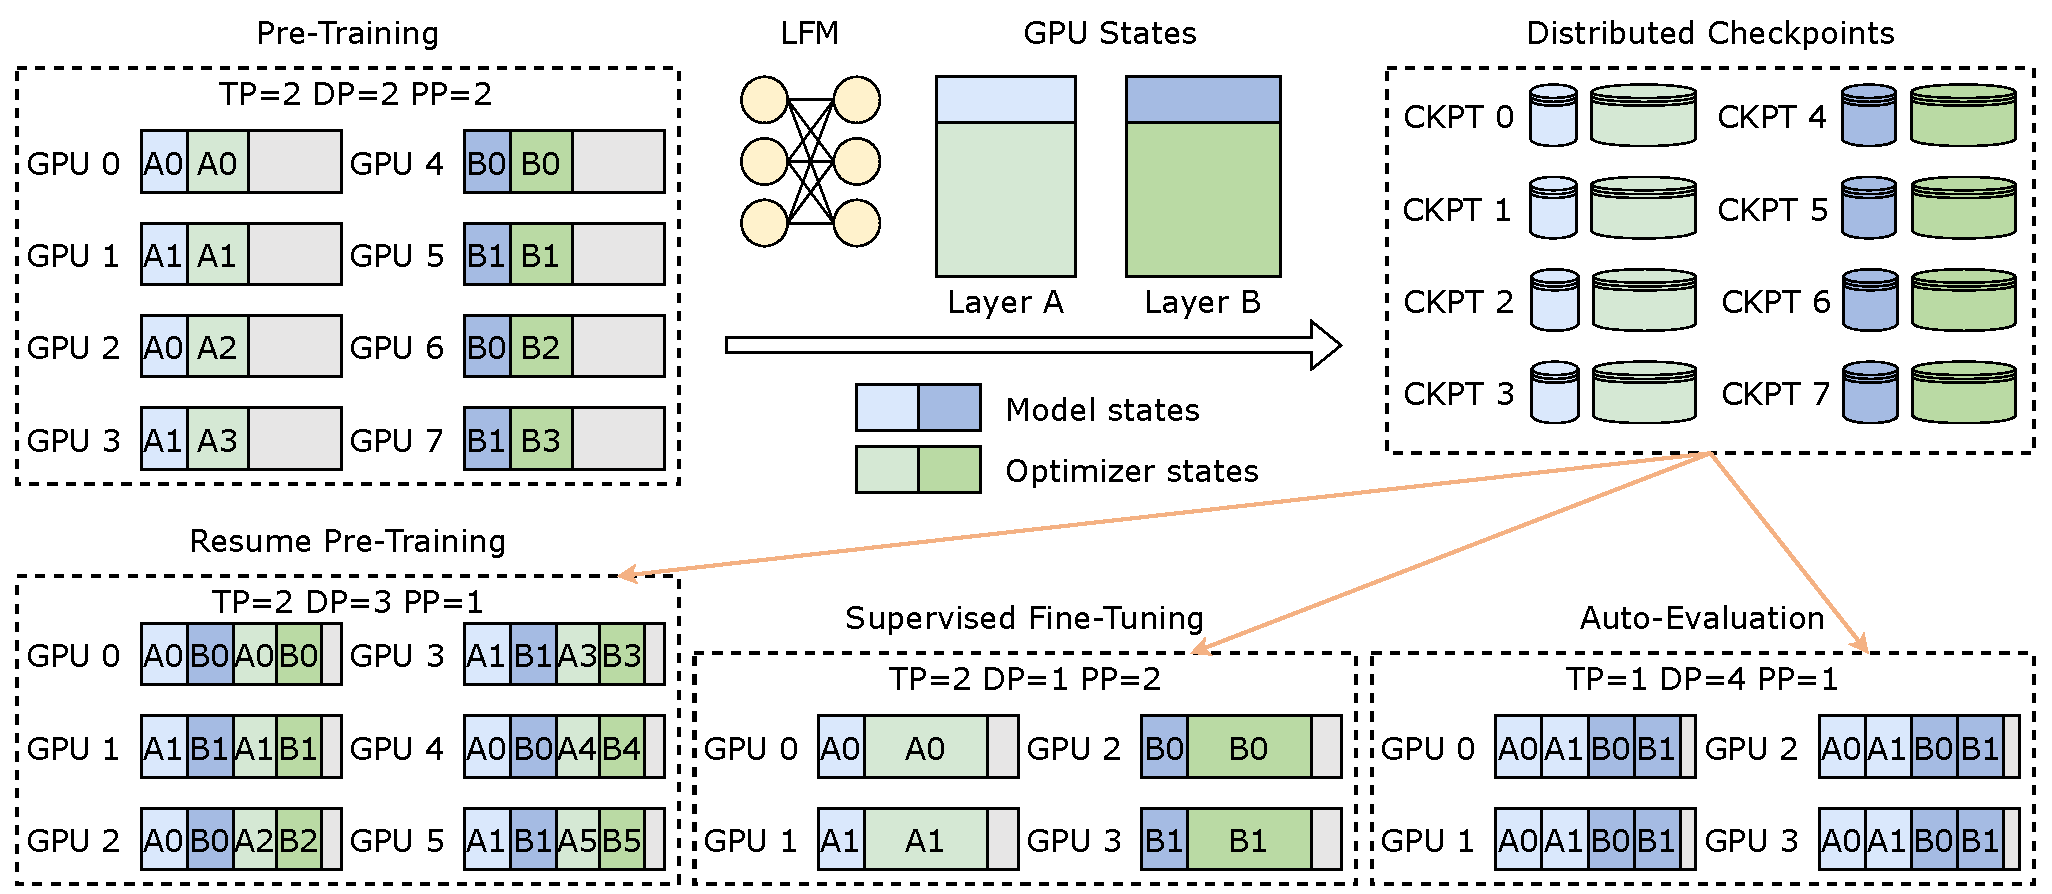
\includegraphics[width=\linewidth]{figures/resharding_requirements.pdf}
  \caption{Checkpoint resharding scenarios in LFM training.
  We only show GPU states for clarity of the figure. %\cwu{explain what the figure shows}
  }
  \label{fig:reshard_req}
\end{figure}

During the life cycle of LFM development, checkpoint resharding is consistently required due to changes in parallelism under different scenarios (Fig.~\ref{fig:reshard_req}):
% (Fig.~\ref{fig:reshard_req}):

\noindent \textit{(1) Training Resumption}.
GPU quota allocated for an LFM training job can vary due to the removal of faulty machines~\cite{megascale, characterization}, adding new machines released from completed tasks, or running on tidal resources~\cite{parcae, qsync, lyra, antman}.
It is often necessary to adjust training parallelism in response to the resource changes, to maximize resource utilization.
Additionally, at the onset of large-scale pre-training, AI engineers often need to experiment with various model configurations and %combinations of 
optimization techniques~\cite{megascale}, since conclusions from small-scale profiling or simulations do not always translate to optimal performance in large-scale training.
In this phase, adjusting parallelism configurations is common, resulting in frequent training resumption.
% continual pre-training such as 
Moreover, long-context training changes the context length, which also requires GPU quota or parallelism adjustment.
% \cwu{explain the distributed checkpoints and `resume pretraining' example in Fig. 2}.
As shown in the example in Fig.~\ref{fig:reshard_req}, 8 distributed checkpoint files are initially stored, then loaded into 6 training workers upon resuming.
% \cwu{briefly explain the auto-evaluation example in the figure.}
%Apart from resharding within one training stage,

\noindent \textit{(2) Cross-Stage Transition}.
When entering 
% transitioning from pre-training to
post-training 
% (\cwu{explain the following in Sec.~2.1 instead} for LLMs, it usually includes supervised fine-tuning~\cite{wei2021sft, wang2022sft} and reinforcement learning from human feedback~\cite{ppo})
, the number of GPUs involved typically decreases due to reduced training data in the latter.
% Different post-training tasks typically use different context window sizes according to their task nature (e.g., multilingual, coding, math, reasoning) and varying GPU resources.
Checkpoints saved from pre-training are frequently resharded to align with the specific workloads of each post-training task.
As depicted in Fig.~\ref{fig:reshard_req}, only 4 GPUs are involved for a fine-tuning task in the post-training stage, so the checkpoints are resharded accordingly.
% \cwu{explain the SFT resharding example in Fig. 2 here}.

\noindent \textit{(3) Evaluation}.
Evaluation tasks in both stages require loading model checkpoints and conducting inference on separate resources;
their parallelism needs to be adjusted to align with assigned GPUs used for specific datasets.
Fig.~\ref{fig:reshard_req} shows a 4-GPU eval task reshards model checkpoints from pre-training.

We collected the number of times of checkpoint resharding demands on our AI platform (training text, image, and video generation models) over the past six months and identified 1,870 instances of checkpoint resharding during pre-training resumption, 13,080 due to cross-stage reconfiguration, and 19,844 for running evaluation tasks. 


\subsection{LFM Checkpointing Requirements}\label{sec:bg_challenges}
% \yhpeng{describe each requirement according to production statistics and why existing ckpt systems do not meet the requirements}
%\subsubsection{Load-time Checkpoint Resharding}
\noindent \textbf{Load-time checkpoint resharding}.
% \noindent \textbf{Ubiquitous resharding requirements.}
% \cwu{the following appears to be more relevant to 2.1 automatic resharding, and little is discussed on saving/loading I/O performance issues}
As a critical step in the life cycle of LFM development, the efficiency of checkpoint resharding is vital to minimize extra overheads.
In our AI platform, the previous common practice is to develop %customized 
offline checkpoint resharding scripts and adapt the scripts whenever a new checkpoint resharding scenario arises.
This approach is inefficient and labor-intensive (see Appendix~\ref{sec:reshard_scripts} for further details).
% Developing and maintaining those scripts, within which the largest one even includes 3193 LoC in Python, are labor intensive.
% since different modules in a given LFM can have different sharding behaviors.
% For example, with Tensor parallelism (TP), Attention and MLP blocks are sharded in different dimensions.
In addition to the development costs, running resharding scripts leads to a substantial waste of GPU time and resources.
Table~\ref{tab:resharding_duration} presents the cost of executing resharding jobs in various scenarios.
Before training can resume or new evaluation tasks can begin, independent jobs that execute the resharding scripts must be submitted in advance.
These jobs download checkpoints from the storage systems, reshard distributed checkpoints to given parallelism configurations and upload new checkpoints back to the storage systems.
The targeted training or evaluation jobs cannot be executed until the completion of resharding jobs, resulting in prolonged pending time.
% For offline resharding executed to resume training (1870.38s on average) a training job must pause until the corresponding resharding job is completed, resulting in considerable wastage of GPU cycles \yiyao {This sentence is a kind of repeat as the one two sentences before}.
Moreover, since checkpoints created by resharding scripts are coupled with specific parallelism, they cannot be reused freely, which in turn increases the storage overhead. 

% The processes of downloading/uploading checkpoint files along with merging and splitting tensor shards in memory incur considerable overheads. 
% Examples of running the offline scripts are given in Fig.~\ref{fig:script_example}. 
% Such offline resharding has several drawbacks.
% Current solution, which is commonly used in industry, is to develop customized resharding scripts (Merging checkpoint could be viewed as a specical case of resharding). However, we observe the significant drawbacks during the development and usages of offline scripts. 

% \textcolor{blue}{The first problem is hard to develop. The resharding logic must be implemented for various model components (such as word embeddings, attention mechanisms, and MLPs) when adjusting different types of parallelism, including tensor parallelism (TP), pipeline parallelism (PP), and data parallelism (DP). For the model, changing the PP alters the layers assigned to each pipeline stage, while changing the TP requires slicing and concatenating tensors according to the previous and current TP degrees. The resharding process for the ZeRO optimizer is even more complex than for the model. Because the ZeRO optimizer flattens TP-sharded tensors and further divides them based on data parallel degrees. Consequently, the resharding scripts for the optimizer require additional logic to handle DP-sharded 1D tensors, on top of the TP/PP resharding logic. } 


% \textcolor{blue}{The second problem is hard to maintain. The field of large foundation models is rapidly evolving, with users frequently implementing and experimenting with novel model structures.  Additionally machine learning systems are continuously exploring new parallelism strategies, such as expert parallelism  and context parallelism which changes the resharding of tensors.  As a result, system developers must update the resharding script each time a new structure or new parallelism style is introduced.Given $K$  model structures and $M$  parallelism strategies, the total number of cases that offline scripts must handle would be  $K \times M$. Maintaining these offline scripts requires significant engineering efforts and costs, as new demands from both algorithm and system sides continue to grow relentlessly. }

% \textit{Next}, offline execution of the resharding scripts leads to substantial GPU time waste.
% \cwu{clarify what checkpoint resharding exactly does so readers can understand why it is CPU and I/O intensive}. %Executing these CPU and I/O-intensive jobs incurs considerable overheads.
%What exacerbates the situation is that the 
% Offline resharding time for training resuming (1870.38s on average) can \cwu{cannot?} be overlapped with concurrent training jobs running on GPU clusters \cwu{but it can be overlapped with other concurrent training jobs?}, 
%due to the existence of non-prearranged 

% As checkpoint resharding requirements arise during training upon unpredictable fluctuations of GPU quotas or experimental algorithm adjustments. % and system performance tuning. In such scenarios, 

Instead of executing scripts in independent jobs for checkpoint resharding, \textit{load-time checkpoint resharding}~\cite{torch-dcp} (also known as online  resharding) is preferred for LFM training.
It automatically identifies and retrieves necessary data from existing distributed checkpoints during the loading procedure.
To achieve this, the storage representation of checkpoints should be designed to be independent of specific parallelism. 
% \cwu{clarify how you can do it in the online way.}

% {The third issue, which only becomes apparent once large-scale training begins, is GPU resource inefficiency during resharding. Running the resharding script to adjust GPU quotas requires only a few machines or GPUs, leaving the GPUs designated for training idle until the resharding process is complete. Training foundation models typically involves at least hundreds of GPUs and can scale up to 10,000 (MegaScale) or even 16,000 GPUs (as with Llama 3.1). Having these GPUs sit idle while waiting for a resharding task that uses far fewer resources leads to significant resource waste. Given that GPUs are the most valuable resource in the era of large foundation models, it is crucial to take action to reduce such waste. }
% Moreover, integrating the checkpoint resharding process into the workflow of various LLM tasks, such as SFT, RLHF, and hyper-parameter tuning adds to the code's complexity, which is not user-friendly.
% conclusion: need a unified representation regardless of specific module implementation.

% Conclusion: unified representation for checkpoints 
%A production-grade checkpointing system must address the inefficiencies associated with offline resharding, design a decoupled representation for checkpoints regardless of the specific implementations of various model (optimizer) modules and parallelism strategies, and thereby enable flexible online checkpoint resharding.

% Unlike checkpointing systems~\cite{checkfreq, check-n-run, gemini-sys, jit-check} that only focus on fault-tolerance and assume constant parallelism configurations, \sys{} enables automatic online checkpoint resharding, shielding users from the intricate transformation logic.

\begin{comment}
\cwu{I commented the table out but described it in text, as the table takes quite some space while not presenting enough information}
\begin{table}[!t]
\caption{
The number of checkpoint resharding requests under different scenarios.
}
\label{tab:resharding_number}
\resizebox{\linewidth}{!}{
\begin{tabular}{ccc}
    \toprule
    \textbf{Resuming} &  \textbf{Evaluation}  & \textbf{Cross-stage Transition}\\
    \midrule
    1870 & 19844  & 13080 \\
    \bottomrule
\end{tabular}}
\end{table}
\end{comment}


% \subsubsection{Supporting multiple training frameworks \& storage backends}
\begin{table}[!t]
\caption{
Average completion time of executing offline resharding jobs under different scenarios.
}
\label{tab:resharding_duration}
\resizebox{\linewidth}{!}{
\begin{tabular}{ccc}
    \toprule
    \textbf{Training Resumption} &  \textbf{Cross-Stage Transition} & \textbf{Evaluation}   \\ 
    \midrule
     1870.38s & 650.34s & 593.21s\\
    \bottomrule
\end{tabular}}
\end{table}

\begin{table}[!t]
\caption{Top three training frameworks used on our platform
}
\label{tab:framework_distribute}
\resizebox{\linewidth}{!}{
\begin{tabular}{cccc}
    \toprule
    \textbf{Framework} & \textbf{Pre-training} &  \textbf{Post-training} & \textbf{Average \#GPUs Per Job 
    % \cwu{per job?}
    } \\ 
    \midrule
    Megatron-LM & 13727& 68621& 301\\
    FSDP & 16842 & $\dagger$ &  25\\
    DDP & 25393& $\dagger$&  6\\
    \bottomrule
\end{tabular}}
\end{table}

\noindent \textbf{Multiple frameworks and storage backends}.
% \noindent \textbf{Support multiple training frameworks and storage backends.}
% 1. Describe the existence of multi-frameworks for different tasks.
On our AI platform, a wide range of training frameworks are used, such as Megatron-LM~\cite{megatron}, DDP~\cite{ddp}, FSDP~\cite{fsdp}, veScale~\cite{megascale, vescale}, etc.
%This variety enables users to make flexible choices based on the specific characteristics and scale of their tasks. 
Table~\ref{tab:framework_distribute} lists the top three preferred training frameworks on our platform, based on six months of trace analysis. %Our experience further reveals that 
Users typically adopt Megatron-LM~\cite{megatron} for training large language foundation models.
FSDP~\cite{fsdp} is preferred for training tasks involving text-to-video or text-to-speech models, 
and DDP~\cite{ddp} is commonly used to train image encoder components of multimodal foundation models or for routine algorithm testing.
In addition, %to selecting training frameworks, 
users can choose from various storage backends for checkpoint persistence depending on the scenario, ranging from local disks for debugging to HDFS or NAS for formal training tasks.
% 2. Describe different tasks that have the same requirements for checkpointing (efficient and async I/O and resharding). 
%Despite the differences, these tasks share common checkpointing requirements, with efficient I/O performance and automatic load-time resharding being the most prevalent.
% 3. Describe the Unique checkpoint module and ad-hoc implementation of different frameworks, separated support requires repeated engineering efforts.
Each training framework comes with its own checkpoint module, file format, and ad-hoc implementation of the save/load logic.
However, these modules lack critical features for production, such as load-time resharding, asynchronous checkpointing, and support for remote persistent storage.
Integrating these features for each framework's checkpoint module and tailoring optimized implementations requires repeated engineering efforts.
This leads to inconsistent checkpointing interfaces across training frameworks and storage backends, complicating the codebase.
Moreover, the maintenance of diverse checkpoint file formats from different frameworks adds to the complexity of implementing checkpoint transfer logic across training stages and deploying models for evaluation and inference tasks.     
Therefore, it is vital to provide generic workflows for different training frameworks and storage backends. 
% Conclusion: unified architecture and checkpointing workflow for training frameworks.

%A production-grade checkpointing system should incorporate a generic execution workflow that supports multiple frameworks and storage backends.
%This not only fulfills the demands of AI researchers but also significantly reduces the development and maintenance costs for system engineers.



\begin{figure}[!t]
  \centering
  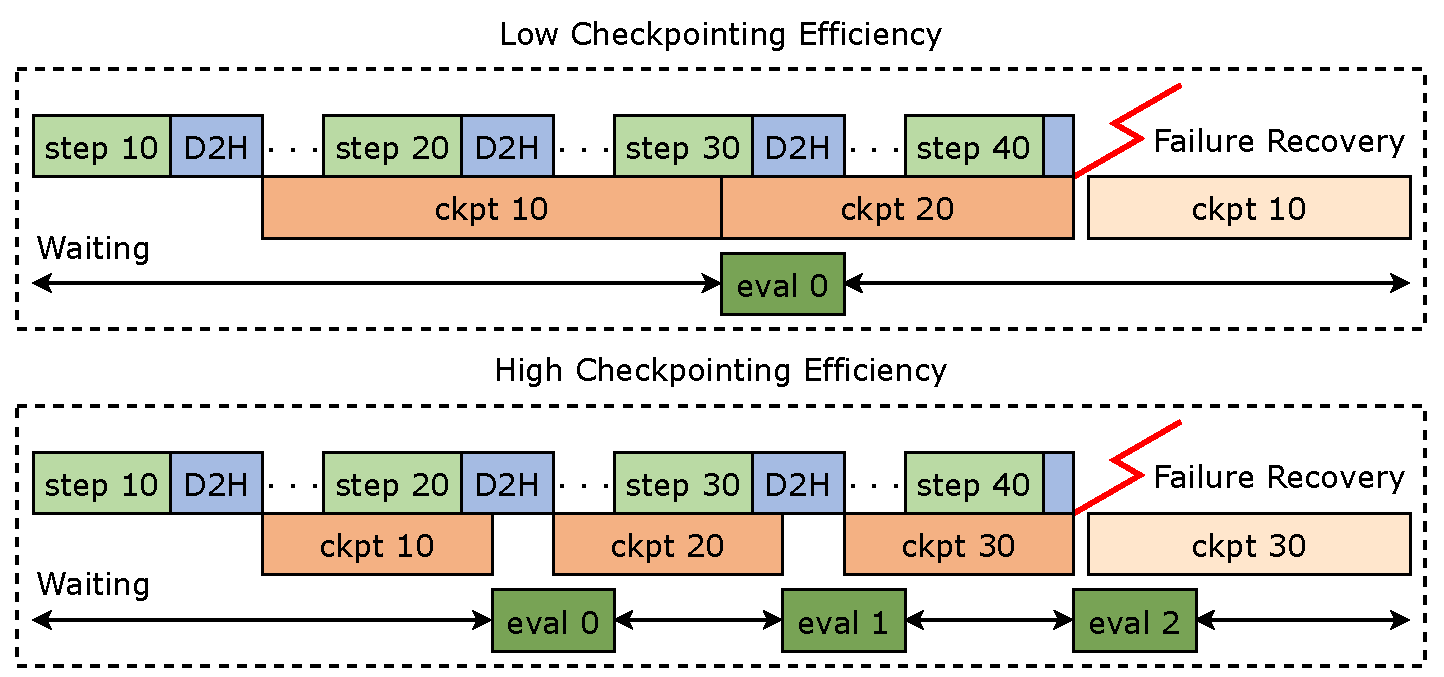
\includegraphics[width=\linewidth]{figures/checkpoint_efficiency.pdf}
  \caption{
  %An illustration of how end-to-end 
  Checkpointing efficiency impacts failure recovery and evaluation tasks.
  D2H denotes the Device-to-Host copy.
  % in checkpointing.
  % \cwu{remove end-to-end from the texts in the figure; clarify what D2H is; not clear what the `Trigger' and the double arrowed lines of evaluation are meant to indicate; the second ckpt 0 in the top figure should be ckpt 10?}
  }
  \label{fig:check_efficiency}
  \vspace{-5mm}
\end{figure}


% Although recent studies have explored in-memory checkpointing~\cite{gemini-sys}, demonstrating significant performance advantages in failure recovery, the necessity for storing checkpoints in persistent storage continues to be crucial in the industry.
%Software and hardware failures are inevitable in large-scale training clusters and no in-memory checkpointing technique can ensure that checkpoints retained in memory will be preserved in the event of various failures.
% The cost of losing training progress in industry-level LLM Pre-Training, which involves substantial data and massive GPU resources, is prohibitively high. 
% Therefore, using persistent storage for checkpointing remains the most reliable and robust method to safeguard training progress and ensure continuity in production environments. \textcolor{blue}{The recent Llama 3.1 [citation] technical report has demonstrated that the training system persists the checkpoint on Tectonic [citation] (Meta's distributed storage system) periodically to reduce the loss of training progress. Additionally, the high failures frequencies and various failure causes making in-memory checkpointing infeasible has showed the necessities of persisting checkpoints. (Mingji) }

 % \textcolor{blue}{Although in-memory checkpointing is intensively studied recently, demonstrating significant performance advantages on failure recovery over checkpointing on persistent storage. We address the necessity of checkpointing on persistent storage.  Software and hardware failures happen inevitably in an industry-level large-scale training cluster. \textbf{None} of in-memory checkpoint techniques can \textbf{guarantee} the checkpoint residing in memory will not be lost when failures happen. The industry-level LLM pre-training uses much data and GPU resources, and the cost of losing training progress is not affordable. Therefore, Checkpointing on persistent storage is the most reliable and defensive way to preserve training progress and production. Second, recovery from failure is just one of the many usage of checkpoint. There are many other demands like auto evaluation on other GPU cluster, training progress rollback, and do fine-tune using other parallelism setting. Snapshoting the checkpoints in the training cluster memory cannot meet these demands. }



%\noindent{\textbf{User expectations on checkpointing}}.
% Design principle. 
% efficiency and reliability are the basic requirements. (Reliability: self-stable and correctness)
% Besides, simple APIs and ease of use also matter. Intuitive APIs, hide the complex logic.
%From our experience, AI researchers and engineers from diverse fields such as computer vision, natural language processing, and speech recognition share the same expectations for underlying checkpointing systems.
%The fundamental requirements are efficiency and reliability.
%All checkpointing-related processing should incur the minimum extra overhead on training workloads.
%Besides, all training states should be safely persisted and correctly resumed, regardless of the changes in parallelism configurations and training environments.
%Users also expect straightforward and intuitive checkpointing APIs that can be seamlessly integrated into their training task pipelines.
%These APIs should shield users from the intricacies of checkpoint management and I/O logic, simplifying integration and enhancing usability across different scenarios.


% AI researchers and machine learning engineers using distributed training frameworks like Megatron-LM, FSDP, or veScale have various expectation on checkpointing sytems. These users require a checkpointing system that is reliable, efficient, and capable with large-scale distributed training. The system should be easy to use while handling the complexities of checkpoint management including, saving, loading, resharding, and merging. \\ Users require efficient and reliable checkpoint saving and resuming capabilities. "Reliability" in this context means that all relevant training states, including the model, optimizer, dataloader, random states, and learning rate scheduler, are persisted correctly and safely. The time required for saving checkpoints should not significantly impede training efficiency. When resuming from checkpoints, users expect all training states to be correctly restored, ensuring consistency with the previous training session. \\The checkpoint system should support resharding of checkpoints when parallelism settings are modified, as well as the ability to merge checkpoints for downstream tasks such as inference or quantization. This flexibility allows users to adapt their checkpoints to various computational configurations and use cases.  \\ Users expect a checkpoint system with a low learning curve. The system should provide simple and intuitive APIs that abstract away the complexities of distributed programming. Furthermore, the underlying system details of resharding and merging should be transparent to users, allowing them to focus on their primary research or development tasks without being burdened by low-level training frameworks or checkpointing system details.
% TODO: add a discussion about iterative development needs resharding.

% \textcolor{blue}{1) When the pre-training or post-training starts, users frequently discover that the parallelism settings estimated from small-scale experiments or simulations do not yield optimal performance in the large-scale training. Adjusting parallelism settings becomes necessary to achieve the best performance and to avoid the waste of GPU resources.}

% \textcolor{blue}{2) In industry training platforms, GPU quotas are dynamic. During a training task, the available GPU quota may increase due to factors such as the addition of new GPUs or the completion of other tasks. Conversely, the available GPU quota may decrease if higher-priority tasks require resources. In both cases, users must reshard the checkpoint and continue training with the new parallelism settings to accommodate these changes.} 

% \textcolor{blue}{3) During the training, the users need to evaulate the model over evaluation datasets periodically to monitor the model quality (auto-evaluation). The auto evaluation tasks with parallelism settings different from training. So users must resharding the checkpoints to the evaluation task can load it correctly. } 

% \textcolor{blue}{4) @borui.wan. Please investigate why SFT needs to change parallism settings frequently}

% We summarize the observed challenges for checkpointing in the industry.



% \begin{table}[!t]
% \caption{
% Time breakdown of running offline checkpoint resharding jobs.
% % For the 100B model, we reshard its checkpoints from TP=a, DP=b, PP=c to TP=A, DP=B, % PP=C;
% % For the 1000B model, we reshard its checkpoints from TP=a, DP=b, PP=c to TP=A, DP=B, % PP=C.
% }
% \label{tab:script_overhead}
% \resizebox{\linewidth}{!}{
% \begin{tabular}{cccc}
%     \toprule
%     \textbf{Model Size} & \textbf{Download Time (s)} &  \textbf{Resharding Time (s)} &%  \textbf{Upload Time (s)}  \\ 
%     \midrule
%     100B & & & \\
%     1000B & & & \\
%     \bottomrule
% \end{tabular}}
% \end{table}


% motivation part: three costs motivate us to design this system.
% 1. High I/O cost during saving/resharding.
% 2. Automatic resharding: Checkpoint merging or offline resharding scripts. 
% 3. Unified system for Checkpoint transfer scripts and efficient checkpoint module to develop.



% Background processing efficiency matters.
% Hardware faults result in failures for checkpoint persistent.
% Intermediate checkpoints are required by auto-triggered accompanying tasks.
% background processing stability matters.
% massive data movement across multiple media, 
% Need to full-stage tracing and monitoring tool and safety mechanism to guarantee the atomic of writing.



% \subsubsection{Efficient checkpoint saving and loading}
% \yhpeng{please describe 1. why offline script is inefficient so we need do it in an online way; 2. why we need high performance and how the saving and loading affect ETTR}
%Given the ubiquity of checkpoint resharding demands during the development of various LFMs, achieving efficient 



% \subsubsection{Efficient and scalable I/O performance}
% \subsubsection{P}
% \noindent \textbf{Achieve efficient and stable I/O performance at scale.}
% Describe massive sizes of LFMs.

\noindent \textbf{Efficient and scalable I/O performance}.
Mainstream LFMs feature extensive model sizes, reaching hundreds of billions of parameters% which can even reach 405B
~\cite{llama3.1}.
%This expansion trend is further fueled by the adoption of sparse structures such as Mixture of Experts (MoE) applied to Mixtral\cite{mixtral}.
Consequently, the size of training states also increases significantly, imposing substantial overhead for checkpoint saving and loading.
% Describe the prolonged time of e2e one-time checkpoint saving.
By analyzing our previous LFM training jobs, we observe that 
the average end-to-end time required to save %distributed 
checkpoints of a GPT 175B model, trained on 4096 GPUs, to HDFS can be 200 seconds.
This duration substantially exceeds the time required for a single training iteration.
% Describe even though existing async checkpointing techniques can removed from the critical path of training, full-stack I/O performance optimizations to cover the whole pipeline of checkpointing are still necessary for 
% 1) Efficient upload efficiency helps mitigate the loss of checkpoint files during training due to frequent hardware failures.
% 2) Auto-triggered accompanying tasks during training like multifaceted evaluation metrics need to wait for the ready of checkpoints of certain steps. Optimization can reduce the blocking of those tasks. 
Even though this time-consuming procedure can be partially removed from the critical path of model training by adopting asynchronous checkpointing~\cite{checkfreq, megascale, reft, datastates-llm}, expediting end-to-end checkpointing remains crucial to minimize training progress loss~\cite{gemini-sys} caused by inevitable frequent failures in large-scale training~\cite{megascale}. 
% (e.g., 466 job interruptions were observed during 54 days of training llama3.1~\cite{llama3.1}).
As depicted in Fig.~\ref{fig:check_efficiency}, although checkpointing overlaps with training, its rapid completion allows more intermediate checkpoints to be stored before a failure occurs, enabling resumption from more recent states and improving ETTR.
Besides, evaluation tasks are triggered during training, and intermediate checkpoints are periodically pulled for these tasks.
Faster checkpointing ensures their timely execution, reducing blocking time due to preparing these checkpoints in remote persistent storage. 
% \brwan{I think use Gemini do not contradict with our motivation}
% \yhpeng{one question from reviewers may be: why not use Gemini that is tailored for failure recovery? any convincing reasons in addition to evaluation tasks? e.g., for short-duration fine-tuning tasks (a few hundred steps, tens of minutes) of large models, ckpt downloading and saving dominates a large percentage of job running time.}
%Inefficient end-to-end checkpointing performance can delay the preparation of these checkpoints in persistent storage, resulting in task blocking.

Scaling the checkpointing system while maintaining the high I/O performance is non-trivial.
Sub-optimal and risky designs, which are hard to detect in small-scale settings, can lead to severe performance bottlenecks or even catastrophic job failures in large-scale training.
For example, massive read/write requests for checkpoint files from the training cluster to the storage systems (e.g., HDFS) can overload the master node, causing delays in file metadata operations.
Additionally, naive implementations of collective communications, such as integrity-checking barriers, introduce substantial initialization and synchronization overheads.
These overheads can even result in communication timeouts, ultimately causing the entire training job to fail.
Furthermore, as training scales up, efficiently analyzing system performance and detecting errors among training and I/O workers across multiple machines becomes increasingly challenging.

Existing checkpointing systems, such as CheckFreq~\cite{checkfreq}, Check-N-Run~\cite{check-n-run}, and Gemini~\cite{gemini-sys}, operate under the assumption of consistent parallelism and do not address the need for checkpoint resharding.
DCP~\cite{torch-dcp} and MCP~\cite{torch-dcp} incorporate checkpoint resharding capabilities but are limited in terms of supported parallelism strategies and training frameworks, I/O performance, and scalability.
% Additionally, both systems exhibit 
% suboptimal I/O performance and scalability issues.
A comprehensive discussion with related works is provided in Appendix~\ref{sec:related_work}.
In \sys{}, we design decoupled storage representation for efficient load-time checkpoint resharding, propose generic saving/loading workflows to support multiple frameworks and storage backends, integrate full-stack optimizations to enhance I/O performance and share our experience in scaling the checkpointing system to support real-world LFM training.
% \cwu{briefly summarize and tell how we are going to meet the above requirements in the paper.}
%A production-grade checkpointing system needs to design full-stack performance optimizations that encompass the entire pipelines of checkpoint saving/loading.
%It should also incorporate monitoring and visualization tools to detect checkpointing exceptions, enabling prompt repairs and guaranteeing system stability.
% Conclusion: 
% 1. Need full-stack I/O performance optimizations to cover the entire pipeline of checkpoint saving/loading to reduce e2e completion time. 
% 2. Need full-stack checkpointing visualization and monitoring toolkits to detect any exceptions and guarantee the atomic of reading/writing.
% The commonly used two-step asynchronous checkpointing~\cite{checkfreq}, adopted by many checkpointing modules~\cite{megascale, torch-dcp, megatron-dcp}, still falls short in terms of efficiency, particularly when dealing with remote persistent storage in large-scale training scenarios.
% \sys{} introduces more refined checkpoint save and load pipelines, incorporating multiple I/O optimization techniques to enhance large-scale checkpointing I/O efficiency.